\documentclass[tikz,border=10pt]{standalone}
\usetikzlibrary{arrows.meta, positioning, calc}
\usepackage{amssymb}

\begin{document}
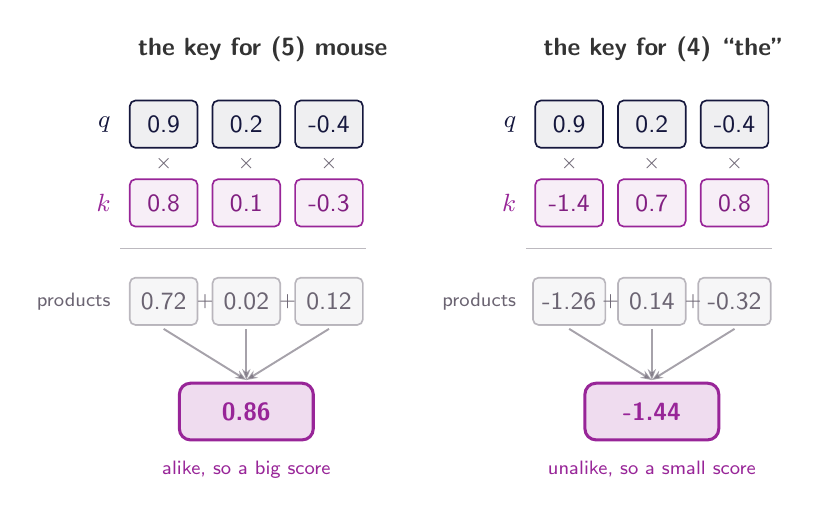
\begin{tikzpicture}[
    every node/.style={font=\sffamily},
]

% ---------------------------------------------------------------- colours
\definecolor{c1}{HTML}{15173D}   % the query
\definecolor{c2}{HTML}{982598}   % the key, and the score it earns
\definecolor{c3}{HTML}{E491C9}
\definecolor{c4}{HTML}{F1E9E9}
\definecolor{axiscolor}{HTML}{333333}
\definecolor{labelcolor}{HTML}{6B6472}   % the intermediate products

\tikzset{
    num/.style={rectangle, minimum width=0.86cm, minimum height=0.6cm,
                font=\sffamily\small, line width=0.6pt, rounded corners=2pt},
    qnum/.style={num, draw=c1, fill=c1!7, text=c1},
    knum/.style={num, draw=c2, fill=c2!8, text=c2!85!black},
    pnum/.style={num, draw=labelcolor, draw opacity=0.45,
                 fill=labelcolor!6, text=labelcolor},
    rowlab/.style={font=\sffamily\small\bfseries, anchor=east},
}

% ================================================================
% Two panels, the same query against two different keys.
%   columns   x = 0, 0.95, 1.9, 2.85   (panel-local)
%   q row     y = 5.2
%   k row     y = 4.2
%   products  y = 2.85
%   score     y = 1.5
% Panel A shifted to x = 0.75, panel B to x = 6.75
% ================================================================

% ----------------------------------------------------------------------
% PANEL A: query against the key for "mouse"
% ----------------------------------------------------------------------
\begin{scope}[shift={(0.75, 0)}]

    \node[font=\sffamily\small\bfseries, text=axiscolor, anchor=west]
        at (-0.45, 6.15) {the key for \textbf{(5)} \emph{mouse}};

    \foreach \v/\i in {0.9/0, 0.2/1, -0.4/2}
        \node[qnum] at (\i*1.05, 5.2) {\v};
    \node[rowlab, text=c1] at (-0.55, 5.2) {$q$};

    \foreach \i in {0,1,2}
        \node[font=\sffamily\scriptsize, text=labelcolor] at (\i*1.05, 4.7) {$\times$};

    \foreach \v/\i in {0.8/0, 0.1/1, -0.3/2}
        \node[knum] at (\i*1.05, 4.2) {\v};
    \node[rowlab, text=c2] at (-0.55, 4.2) {$k$};

    \draw[labelcolor, opacity=0.45, line width=0.6pt]
        (-0.55, 3.62) -- (2.57, 3.62);

    \foreach \v/\i in {0.72/0, 0.02/1, 0.12/2}
        \node[pnum] at (\i*1.05, 2.95) {\v};
    \node[font=\sffamily\scriptsize, text=labelcolor, anchor=east]
        at (-0.55, 2.95) {products};

    \foreach \i in {0,1}
        \node[font=\sffamily\scriptsize, text=labelcolor] at (\i*1.05+0.525, 2.95) {$+$};

    \foreach \i in {0,1,2}
        \draw[-{Stealth[length=4pt]}, line width=0.7pt, labelcolor, opacity=0.6]
            (\i*1.05, 2.6) -- (1.05, 1.95);

    \node[rectangle, rounded corners=4pt, minimum width=1.7cm,
          minimum height=0.72cm, draw=c2, line width=1.1pt, fill=c2!16,
          font=\sffamily\small\bfseries, text=c2] at (1.05, 1.55) {0.86};
    \node[font=\sffamily\scriptsize, text=c2, anchor=north] at (1.05, 1.05)
        {alike, so a big score};

\end{scope}

% ----------------------------------------------------------------------
% PANEL B: the same query against the key for "the"
% ----------------------------------------------------------------------
\begin{scope}[shift={(5.9, 0)}]

    \node[font=\sffamily\small\bfseries, text=axiscolor, anchor=west]
        at (-0.45, 6.15) {the key for \textbf{(4)} \emph{``the''}};

    \foreach \v/\i in {0.9/0, 0.2/1, -0.4/2}
        \node[qnum] at (\i*1.05, 5.2) {\v};
    \node[rowlab, text=c1] at (-0.55, 5.2) {$q$};

    \foreach \i in {0,1,2}
        \node[font=\sffamily\scriptsize, text=labelcolor] at (\i*1.05, 4.7) {$\times$};

    \foreach \v/\i in {-1.4/0, 0.7/1, 0.8/2}
        \node[knum] at (\i*1.05, 4.2) {\v};
    \node[rowlab, text=c2] at (-0.55, 4.2) {$k$};

    \draw[labelcolor, opacity=0.45, line width=0.6pt]
        (-0.55, 3.62) -- (2.57, 3.62);

    \foreach \v/\i in {-1.26/0, 0.14/1, -0.32/2}
        \node[pnum] at (\i*1.05, 2.95) {\v};
    \node[font=\sffamily\scriptsize, text=labelcolor, anchor=east]
        at (-0.55, 2.95) {products};

    \foreach \i in {0,1}
        \node[font=\sffamily\scriptsize, text=labelcolor] at (\i*1.05+0.525, 2.95) {$+$};

    \foreach \i in {0,1,2}
        \draw[-{Stealth[length=4pt]}, line width=0.7pt, labelcolor, opacity=0.6]
            (\i*1.05, 2.6) -- (1.05, 1.95);

    \node[rectangle, rounded corners=4pt, minimum width=1.7cm,
          minimum height=0.72cm, draw=c2, line width=1.1pt, fill=c2!16,
          font=\sffamily\small\bfseries, text=c2] at (1.05, 1.55) {-1.44};
    \node[font=\sffamily\scriptsize, text=c2, anchor=north] at (1.05, 1.05)
        {unalike, so a small score};

\end{scope}

% the takeaway lives in the figcaption, not inside the figure

\end{tikzpicture}
\end{document}
